\chapter{Lezione 6 - Attori e regole del web}

Argomenti:

\begin{itemize}
    \item Gli attori del web 2.0
    \item la contestazione dei nomi a domenio
    \item le regole di netiquette
\end{itemize}
In una lezione precedente abbiamo raccontato la storia del web dalle origini fino ad oggi. Il passaggio soprattutto da un web 1.0 al web 2.0 che è il web a cui siamo di fronte in questi in questi anni.\par
Chi sono gli attori di questo web 2.0 e in che modo interagiscono fra di loro?
\section{Attori del web 2.0}
Il web è una parte integrante della vita comune delle persone ed è caratterizzato da:
\begin{itemize}
    \item un linguaggio di comunicazione comune per l'accesso di dispositivi diversi
    \item da sistemi e strutture di coordinamento per l'identificazione e la raggiungibilità dei dispositivi e quindi degli utenti. 
\end{itemize}

Facciamo un passo indietro. Nel periodo che va dal 1991, data nella quale sono state pubblicate le prime pagine web e in cui il web divenne pubblico e sino ai primi anni 2000 gli utenti interagivano attraverso la rete in maniera sostanzialmente passiva. Sono anni in cui si iniziava a sperimentare la rete internet perché precedentemente, prima degli anni 90, la rete era dedicata e utilizzata soltanto da esperti informatici appartenenti alle università e prima ancora all'ambiente militare degli Stati Uniti. \par
Nel primo periodo in cui il grande pubblico ha avuto accesso ad internet l'interazione riguardava essenzialmente l'utilizzo di documenti elettronici e l'invio di messaggi di post elettronica.\par Successivamente comparvero le prime forme di comunicazione digitale più moderne parliamo di newsgroup o forum che erano sostanzialmente dei salotti di discussione digitale ed è attraverso queste forme di interazione che ha cominciato a svilupparsi una vera e propria interazione di massa mai avvenuta prima tra utenti inesperti.\par
Dopo il 2000 nasce il web 2.0.
Dal 2004-2005 due sono i concetti chiave:
\begin{itemize}
    \item la condivisione dei contenuti multimediali 
    \item la partecipazione attiva degli utenti nella gestione 
    \item 
\end{itemize}

  Anche il web 2.0 nasce negli Stati Uniti, tra il 2004 e il 2005 un grande editore americano o Riley Media organizzò una serie di conferenze per spiegare le nuove opportunità della comunicazione e per spiegare che la rete internet e in particolare il web metteva a disposizione degli utenti non esperti in informatica una serie di strumenti che permettevano appunto a questi utenti non esperti di partecipare attivamente e di gestire in modo autonomo i contenuti multimediali. \par
  Durante questi incontri si coniò il concetto di web 2.0 che da allora fu utilizzato costantemente e l'elemento essenziale del web 2.0 è proprio il fatto che è possibile un'interazione avanzata non solo tra esperti informatici ma anche tra persone comuni, utenti non esperti. \par
  Potete vedere in questa immagine un confronto delle interazioni che hanno avuto luogo nella prima fase del web il web 1.0 e il web 2.0.
  
  \begin{figure}[h]
      \centering
      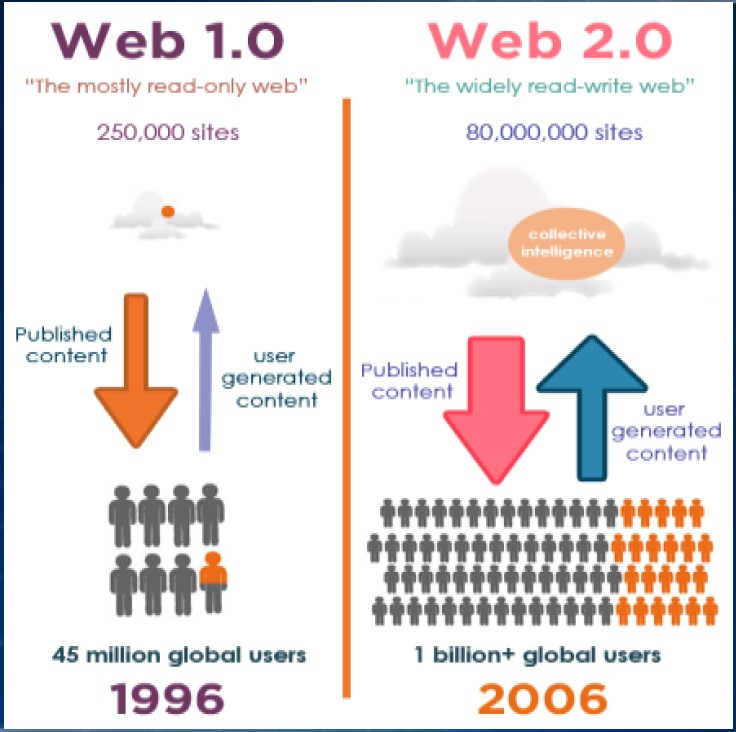
\includegraphics[width=0.75\linewidth]{images/06_lez_fig_01.jpg}
  \end{figure}
  
  Nel 1996 gli utenti globali di internet erano 45 milioni, nel 2006 a distanza di dieci anni oltre un miliardo di utenti di internet e anche la gestione dei contenuti è cambiata. I contenuti pubblicati da soggetti specializzati rispetto ai contenuti generati dagli utenti hanno un rapporto completamente diverso nel 1996 e nel 2006. Anche i siti presenti sul web 250 mila nel web 1.0, 80 milioni nel web 2.0. Si vede la grandissima differenza che nell'arco di dieci anni ha caratterizzato il rapporto dei cittadini con il web.\par
  Per stare sul web occorre un dispositivo, i dispositivi oggi che consentono di approcciarsi al web sono innumerevoli, parliamo di tablet, di smartphone, di pc, di laptop e poi occorre un luogo su cui inserire i contenuti. Questo luogo può essere un sito creato da altri oppure un proprio sito e per avere un proprio sito occorre assicurarsi un dominio e per questo ci si rivolge ad un provider che generalmente offre servizi legati all'apertura del dominio ma anche altri servizi come un indirizzo email e lo spazio web necessario per creare il proprio sito.\par 
  Ricorderete dalle lezioni precedenti che il dominio è raggiungibile attraverso l'indicazione di un codice numerico ma che nel contesto del web questo codice numerico è sostituito da un nome vero e proprio, in maniera tale da semplificare e facilitare all'utente il ricordo di qual è la destinazione che vuole raggiungere.\par
  Per poter effettuare la registrazione di un dominio, deve esserci un fornitore e questo deve essere riconosciuto come registrar ufficiale. Tutti i registrar che si occupano di domini.it lavorano insieme al NIC italiano, il registro .it, che è l'organo di registrazione centrale di tutti gli indirizzi italiani. Il NIC italiano fa riferimento all'ICANN che coordina la distribuzione dei domini di tutto il mondo.\par
  Entrambe queste organizzazioni e le altre organizzazioni che sono attori all'interno del web, come operano davvero e come funziona concretamente l'assegnazione dei domini?\par
  Riprendiamo quindi adesso più nel dettaglio un argomento che abbiamo iniziato ad affrontare in una lezione precedente.\par 
  \section{ICANN}
  ICANN è l'Internet Corporation for Assigned Names and Numbers ed è responsabile per l'assegnazione e la gestione degli indirizzi web di primo livello, i General Top Level Domain. ICAN coordina tutti gli indirizzi web esistenti e assicura che ogni dominio sia unico, identificabile in maniera inequivocabile e raggiungibile attraverso un browser. Tuttavia non si occupa direttamente dell'assegnazione di questi indirizzi.\PAR
  \begin{itemize}
      \item E' stato istituito nel 1998 su incarico delle autorità governative degli USA. 
      \item ICANN oggi è un ente di gestione internazionale del quale fanno parte diverse entità non solo americane ma anche europee. 
      \item ICANN, come detto, ha l'incarico di assegnare gli indirizzi IP e identificare e gestire i General Top Level Domain nel mondo.
      \item 
  \end{itemize}
   \par
  ICAN è coadiuvato da altri soggetti in particolare il NIC Registry.

  \subsection{NIC Registry}

\begin{itemize}
    \item NIC Registry ovvero Network Information Center o Domain Name Registry che sono autorizzati da ICANN 
    \item Si tratta di Naming Authorities che:
    \begin{itemize}
        \item gestiscono la registrazione dei domini locali o di secondo livello che sono
        \item responsabili del servizio WHOIS
    \end{itemize}  
    
\end{itemize}
  
  Ricorderete che i domini generali di secondo livello sono i Country Code Top Level Domain e sono quelli caratteristici dei diversi paesi nel mondo. Quindi abbiamo .it, .fr, .uk a seconda del paese di appartenenza a cui fanno riferimento. \par
  I Registry associano gli indirizzi numerici necessari per muoversi in rete che sono lunghi e difficili da memorizzare con un nome. I registry a loro volta sono supportati da altri soggetti.
  \subsection{Domain Name Registrar}
  I Domain Name Registrar sono partner del NIC e si occupano della registrazione del dominio. 
  Provvedono a chiedere i dati relativi al registrante e li raccolgono in un database, il database proprio dei nomi di dominio e questo database contiene tutte le informazioni relative a coloro che chiedono e ottengono la registrazione di un nome di dominio. Il database che contiene i dati dei registranti può essere consultato attraverso un servizio che si chiama WHOIS (chi è).
  
  I Domain Name Registrar
  \begin{itemize}
      \item gestiscono la registrazione dei nomi locali o di secondo livello 
      \item sono responsabili del servizio WHOIS 
      \item 
  \end{itemize}{}
  
   Per quanto riguarda l'Italia, il riferimento di ICANN è il registro.it. 
   \subsection{registro.it}
    Il registro .it:
   \begin{itemize}
       \item stabilisce in autonomia i criteri di assegnazione dei domini IT 
       \item gestisce e amministra i top level domain .it 
       \item gestisce i nomi dei server che consentono la raggiungibilità dei siti web .it 
   \end{itemize}
   
   Il registro è gestito dal Consiglio nazionale delle Ricerche e ha sede presso l'Istituto di Informatica e Telematica del CNR di Pisa, del Centro nazionale delle Ricerche di Pisa.\par
   Il registro .it è l'anagrafe dei domini .it, la targa internet dell'Italia. Soltanto attraverso di esso è possibile richiedere, modificare o cancellare uno o più domini .it.\par
   Il registro.it:
   \begin{itemize}
       \item come tutti i domini nazionali, si affida a registrar autorizzati 
       \item gestisce il database dei nomi assegnati 
       \item offre il servizio WHOIS .it
   \end{itemize}
    
    Attraverso il servizio WIS si ottengono informazioni sulla disponibilità del dominio e sul suo eventuale proprietario. In questo modo sono messi a disposizione del server di tutti i domini che hanno la stessa estensione insieme ai loro indirizzi IP. 
    %%11:37
    \subsubsection{3WC Consortium}
    
    Un altro attore del web è il 3WC Consortium, il World Wide Web Consortium. Si tratta di un'organizzazione internazionale nata nel 1994, è un'organizzazione non governativa ed è nata presso il MIT, il Massachusetts Institute of Technology, inventata dal padre del web, Tim Barners-Lee, in collaborazione con il CERN. \par
    Il 3WC ha come scopo quello di sviluppare le tecnologie che garantiscono l'interoperabilità, le specifiche tecniche, le guideline e le linee guida delle applicazioni. L'obiettivo è quello di portare il World Wide Web al massimo del suo potenziale, agendo da forum internazionali con comunicazioni e attività comuni. \par
    La composizione del 3WC Consortium è molto variata, è composto da aziende informatiche multinazionali di diversi settori, università e centri di ricerca. È inoltre un soggetto a cui compartecipano gli Stati Uniti e l'Unione Europea. \par
    Il 3WC Consortium ha l'obiettivo di garantire il libero accesso al web. Per riuscirci è necessario, come detto, elaborare dei criteri comuni di utilizzo, un linguaggio comune condiviso di utilizzo, perché se ci fossero linguaggi diversi sarebbe ovviamente difficile poter interagire. Quindi il 3WC promuove:
    \begin{itemize}
        \item standard tecnici comuni 
        \item interoperabilità 
        \item sviluppo di nuovi linguaggi 
    \end{itemize}
    
    L'importanza dei membri del 3WC Consortium è tale che ne fa un organismo di grande autorevolezza. 
    
    
    \subsubsection{utenti del web 2.0}
    Gli ultimi attori del web ma determinanti nel web 2.0, sono gli utenti. 
    Gli utenti del web 2.0 hanno a disposizione strumenti che con la loro duttilità e semplicità d'uso sono a disposizione dell'utente non esperto per consentirgli di operare. Sul web 2.0 molti nuovi servizi, la gran parte gratuiti, generano degli strumenti mediatici di grande potenzialità. Il loro utilizzo non richiede alcuna competenza specifica. Alcuni di questi servizi sono sviluppati interamente dagli utenti e non più dai tecnici e quindi hanno cambiato completamente pelle.
    
    Vediamo adesso un breve video per riepilogare in qualche modo quello che abbiamo detto fino ad ora.
    \par
    \textit{Nel video si parla dell'interazione utenti web 2.0 (Facebbok, Twittwr, youtube, ecc) e della possibilità di fare marketing. E' molto breve.}\par
    
    Avete visto quali sono gli strumenti messi a disposizione al giorno d'oggi, ma cerchiamo di capire un po' più nel dettaglio. \par
    Gli utenti possono utilizzare una serie di strumenti diversi:
    \begin{itemize}
        \item Wiki sono sistemi sviluppati e modificati liberamente dagli utilizzatori. Il caso esemplare di questo tipo di servizi è rappresentato da Wikipedia, l'enciclopedia libera sulla quale ogni utente iscritto può generare contenuti e che possono essere modificati e implementati da chiunque abbia accesso. Si tratta di un'enciclopedia libera e gratuita che nel bene o nel male è diventata un punto di riferimento per tutti coloro che fanno ricerche in rete ed è come detto interamente redatta dagli utenti che la utilizzano
        \item I CMS, Content Management System, sono dei sistemi di gestione dei contenuti multimediali e sono dei modelli di siti web preconfezionati per i quali basta scegliere un tema grafico da utilizzare e poi appunto riempirlo di contenuti. I CMS dispongono anche di funzionalità avanzate come la gestione degli utenti iscritti al blog e la gestione dei loro commenti e degli articoli pubblicati da altri
        \item I Feed RSS sono aggregatori di notizie, di articoli su argomenti specifici, di account email, di commenti sugli articoli dei blog e così via. Raccolgono le informazioni su vari siti differenti. Quando si avviano o vengono aggiornati questi programmi, le pagine web che ci interessano, già predisposte per l'uso, trasferiscono sul lettore Feed RSS una lista di articoli alla quale è possibile accedere rapidamente.
        \item I Cloud Computing. Il Cloud Computing è un insieme di tecnologie e di servizi che ci consentono di memorizzare i nostri dati, dati che utilizziamo per lavorare e quant'altro su un archivio multimediale, un archivio che è esterno al nostro computer e che risiede su un server da qualche parte nella rete internet. Con questa tecnologia tutti i documenti che elaboriamo vengono conservati su uno spazio web personalizzato senza occupare la memoria dei dispositivi che sono a nostra disposizione per l'archiviazione dei dati e senza impegnare il nostro sistema operativo. Il cloud permette di lavorare senza installare alcun software e di usufruire dei programmi e di altre risorse di cui abbiamo bisogno direttamente usando la rete. Il cloud, così come alcuni degli altri strumenti che sono a disposizione, hanno delle caratteristiche che possono anche presentare delle difficoltà ma ci occuperemo in una prossima lezione di quali sono le questioni più strettamente giuridiche collegate a questi sistemi.
        \item I social media sono gli strumenti di comunicazione sulla rete più diffusi in assoluto e più utilizzati e consentono l'interazione tra un grandissimo numero di utenti, tra i più noti Facebook che ha fatto in qualche modo da padrone nell'arco di dieci anni e che nella primavera del 2018 è stato coinvolto in uno scandalo molto grande, con molti effetti, che è il cosiddetto scandalo Cambridge Analytica e che ha riguardato la creazione e l'utilizzo di falsi profili su Facebook rubati da persone vere ed esistenti con finalità che erano collegate alle elezioni del presidente Trump negli Stati Uniti nel 2017. Ma anche di questo parleremo in una prossima lezione meglio. 
    \end{itemize}

    \textit{Lo scandalo dei dati Facebook-Cambridge Analytica[1] è stato uno dei maggiori scandali politici avvenuti all'inizio del 2018, quando fu rivelato che Cambridge Analytica aveva raccolto i dati personali di 87 milioni di account Facebook senza il loro consenso e li aveva usati per scopi di propaganda politica.[2] È stato definito come un momento di spartiacque nella comprensione pubblica del valore dei dati personali e di conseguenza, provocando un forte calo del prezzo delle azioni di Facebook, si è chiesto una regolamentazione più rigorosa sull'uso dei dati personali da parte delle aziende tecnologiche.[3]
    Lo scandalo scoppiò a marzo 2018 a causa delle rivelazioni di un whistleblower, un ex dipendente della Cambridge Analytica, Christopher Wylie.}
    
        
     
      Vediamo adesso però qual è la penetrazione nel mondo al giorno d'oggi, nel 2018. 
      
      \begin{figure}[h]
          \centering
          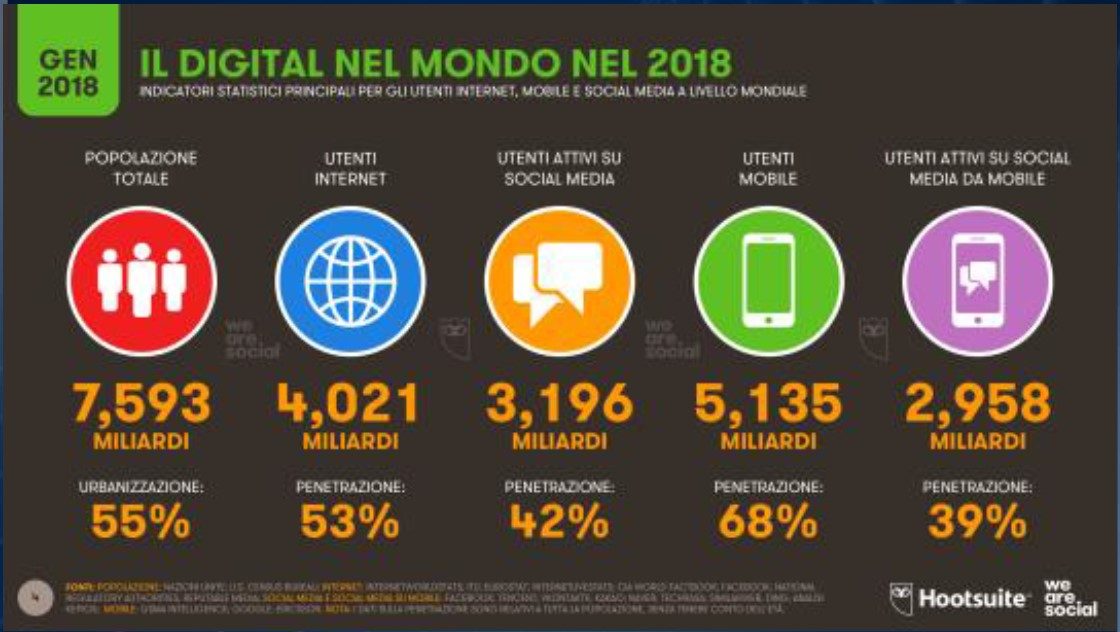
\includegraphics[width=0.75\linewidth]{images/06_lez_fig_02.jpg}
      \end{figure}
      
      Il digital nel mondo del 2018. Ecco qui da questo studio del 2018 potete vedere la penetrazione della rete nella popolazione totale. Abbiamo una popolazione totale di 7 miliardi e mezzo di persone, un'urbanizzazione del 55\% e 4 miliardi e abbondanti di utenti internet con una penetrazione del 53\%. \par
      Tra gli utenti di internet attivi sui social media sono più di 3 miliardi, utenti mobile sono più di 5 miliardi e utenti sui social media da mobile sono quasi 3 miliardi. \par
      
      \begin{figure}[h]
          \centering
          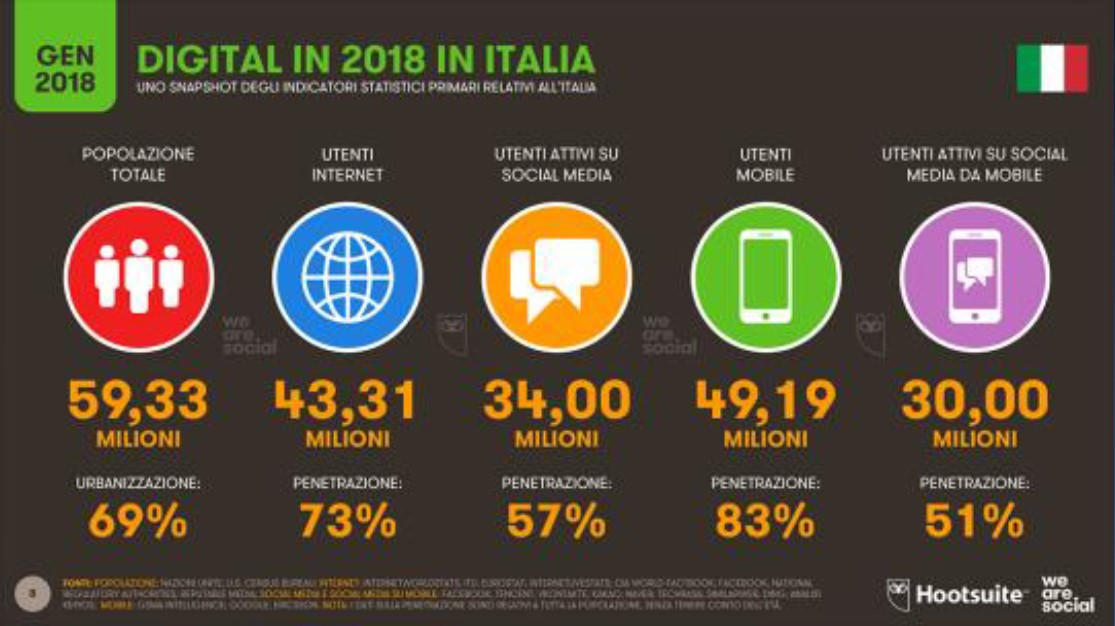
\includegraphics[width=0.75\linewidth]{images/06_lez_fig_03.jpg}
      \end{figure}
      
      In Italia dal gennaio 2018 abbiamo delle percentuali di presenza sul web estremamente elevate. Su 59 milioni di popolazione locale abbiamo 43 milioni di utenti internet. \par
      Quindi come potete vedere ormai nel 2018 internet è diffuso ovunque. Se pensate a come era la situazione nei primi anni 90 dello scorso secolo, ricorderete abbiamo esaminato una timeline in una delle precedenti lezioni nelle quali proprio si comprendeva qual è stato il passaggio per il mondo moderno dall'epoca degli inizi di internet fino a oggi al web 2.0. \par
      Potete rispondere ad una domanda. Come è cambiato il ruolo dell'utente nel web 2.0?
      
      \subsection{Contestazione dei nomi a dominio.}
      \subsubsection{Regole di assegnazione dei nomi a dominio}
      Passiamo ad un altro argomento. Il nostro argomento adesso è contestazione dei nomi a dominio. 
      \subsubsection{Regole di assegnazione dei nomi a dominio}
      La regola di base è first come first served, ma questa regola non tiene conto del fatto che può esserci un problema:
      \begin{itemize}
          \item di diritto d'autore 
          \item o può esserci un diritto all'uso del nome o della denominazione che non è quello di chi cerca di registrare il dominio. 
      \end{itemize}
        Il registro infatti non fa delle verifiche sulla effettiva titolarità del nome che si vuole registrare.   \par 
      Se le regole sono violate, la persona che ha diritto ad utilizzare un determinato nome e che si rende conto che è stato utilizzato da altri ha degli strumenti diversi per riottenere l'assegnazione del nome a dominio a se stesso.\par
      
      Perché un principio di chi primo arriva meglio alloggia è utilizzato sul web? Per una questione da un lato di praticità e rapidità, dall'altro perché come avete visto i domini sono assegnati da diversi registrar e quindi diventa estremamente difficile poter verificare se chi fa la richiesta di registrazione ha dei diritti effettivi e non calpesta invece i diritti degli altri. Nella registrazione è comunque richiesto di autodichiarare di avere i diritti per utilizzare quel determinato nominativo ma una verifica non viene fatta. Cosa può fare l'utente? L'utente può contestare il nome a dominio. 

      \subsubsection{Contestare i nomi a dominio}
      
      L'assegnazione di un dominio dunque può essere controversa tra diversi soggetti. 
      \begin{itemize}
          \item Può esserci un diritto prioritario sul nome a dominio legato a un marchio registrato , all'esistenza di un determinato cognome e così via
          \item è possibile invece che il titolare del dominio lo abbia registrato utilizzando il nome a fini speculativi o abusivi
      \end{itemize}

      %24:31
      Come contestare i nomi a dominio? 
      \begin{itemize}
          \item Esistono procedure di contestazione regolate e gestite dai registri locali 
          \item devono tener conto dell'applicazione della normativa locale 
          \item 
      \end{itemize}
      
       Per contestare i nomi a dominio è possibile fare una \textbf{opposizione} che consente l'accesso a due procedure alternative al ricorso alla magistratura per la risoluzione della controversia. \par
       L'opposizione di per sé non permette la riassegnazione automatica del dominio già registrato da altri però consente di attivare questo processo che è un processo stragiudiziale per ottenere e far valere le proprie ragioni. \par
       Quindi contestare i nomi a dominio comporta la possibilità di fare una opposizione a cui segue: 
       \begin{itemize}
           \item un arbitrato irrituale 
           \item oppure una procedura di riassegnazione 
       \end{itemize}
       
Al termine della procedura viene effettivamente riassegnato il dominio. \par 
L'arbitrato irrituale consiste nell'affidare ad un collegio di persone esperte nell'assegnazione dei nomi a dominio la questione lasciando a loro di valutare, sulla base di una rapida istruttoria, chi abbia effettivamente il diritto di utilizzare quel determinato nome. Per poter accedere a questa procedura il registrante deve però aver sottoscritto la clausola arbitrale. \par 
La procedura di riassegnazione invece anche questa è condotta da soggetti privati, sono degli studi professionali chiamati prestatori del servizio di risoluzione delle dispute (PSRD) e ha anche qui lo scopo di verificare che il dominio non sia stato registrato e mantenuto in mala fede. L'unico esito della procedura è la riassegnazione del dominio al soggetto che ha iniziato l'opposizione.\par 
       
Per la gestione delle dispute ogni registro adotta delle regole simili. Per quanto riguarda l'Italia è il registro.it che provvede alla non solo all'assegnazione dei nomi di dominio ma anche a dirimere le controversie, per quanto riguarda l'Europa le informazioni sulla riassegnazione dei nomi a dominio e sulle procedure di opposizione si trovano sul sito di eurid.eu.it.\par 

Lo spunto di riflessione di questa parte della nostra lezione è quali procedure si possono attivare per contestare un nome a dominio.it?

\section{Le regole di netiquette}

Le regole di netiquette. Alle origini e per lungo tempo internet non era regolato in alcun modo. Ricordiamo ancora una volta che alle origini e per i primi anni l'accesso a internet era possibile ad un numero limitato di utenti che erano sostanzialmente esperti o appartenenti a determinate categorie. Ma già dall'inizio degli anni 90 dello scorso secolo vi è stata l'apertura agli utenti comuni con un conseguente aumento di presenze sulla rete. Siamo passati dall'internet al web e così via. E' stato avviato un percorso che ancora non si è concluso.\par
Nei primi anni appunto non c'era nessun tipo di regolamentazione sul web ma l'esigenza di qualche forma di regolamentazione fra gli utenti si è sentita quasi dalle origini.\par 
La netiquette consiste in un insieme di regole di buona educazione in rete. Come nasce questa parola? Da net (network, rete) e etiquette (buona educazione in lingua francese). La netiquette non è un regolamento imposto dall'esterno ma è una forma di autoregolamentazione degli utenti che ancora oggi valida anche se nel frattempo alcune norme sono state elaborate.\par
La netiquette, le regole di buona educazione sono sempre valide e sono sempre applicabili anche se non spesso utilizzate.\par
\textbf{La netiquette è un insieme di regole informali che disciplinano il buon comportamento dell'utente di internet (nel rapportarsi con gli altri utenti).}\par
\subsubsection{RFC 1855}
Come sono nate queste regole? Nel 1995 fu fatto una richiesta di commenti pubblicata, request for comment (RFC). Queste regole sono costituite da:

\begin{itemize}
    \item buona prassi 
    \item vietano comportamenti scorretti
    \item vietano la commissione di reati 
\end{itemize}

Sono ancora reperibili sul sito dove in origine sono state pubblicate. (https://tools.ietf.org/html/rfc1855) netiquette guidelines.\par

\subsubsection{il buon netizen}

Nel rfc 1855 sono elencate tutte le regole che permettono di diventare un buon netizen.\par 
Quali sono le regole che deve rispettare? 
Bisogna distinguere i vari tipi di comunicazione:
\begin{itemize}
    \item Comunicazione a uno a uno (post elettronica e dialogo) 
    \item Comunicazione uno a molti tramite blog, social network, instant messenger 
    \item servizi di informazione più generali 
\end{itemize}

Le regole di base:
\begin{itemize}
    \item non appropriarsi di contenuti di altri 
    \item non pubblicare il contenuto di un messaggio e email senza consenso 
    \item non fare spam
    \item non violare la sicurezza
    \item non violare la privacy
    \item non compromettere il funzionamento della rete
\end{itemize}

Come potete notare si tratta di regole che in gran parte sono comunque presidiate da norme internazionali e nazionali, sia la tutela della privacy, sia la tutela rispetto alla commissione di crimini informatici, sia la tutela del diritto d'autore e così via. La maggior parte delle regole del buon vivere civile sulla rete sono regole che hanno un presidio offline forte con delle norme nazionali e internazionali e che quindi rispettare le regole di buona educazione porta anche a rispettare le leggi.\par 
Oltre a queste regole di base ci sono delle indicazioni specifiche legate al tipo di interazione. \par
Nell'interazione da uno a uno:
\begin{itemize}
    \item si suggerisce nel testo di limitare l'uso del maiuscole e del grassetto 
    \item si suggerisce di avere sintesi evitando divagazioni inutili 
    \item si suggerisce di inviare le proprie comunicazioni a dei destinatari limitati e effettivamente necessari 
\end{itemize}

Il suggerimento è quello di evitare di urlare sul web come può accadere invece con l'abuso di strumenti di evidenziazione e di richiamo.\par 
Nel caso dell'interazione da uno a molti:
\begin{itemize}
    \item si parla di newsgroup e liste di distribuzione e si suggerisce di leggere prima di scrivere 
    \item limitare e fare attenzione a ciò che viene inviato in cc e in ccn, in copia evidente e in copia nascosta. Ad esempio è opportuno utilizzare il ccn che non permette a tutti gli altri di conoscere gli indirizzi di posta elettronica della lista di destinatari per questioni di riservatezza. 
    \item Si suggerisce di fare citazioni chirurgiche, fatte bene e con indicazione della fonte 
    \item evitare guerre di opinioni in rete 
    \item non inviare messaggi pubblicitari inutilmente
\end{itemize}

Anche in questo caso le regole sono abbastanza semplici, non sempre vengono ricordate. Negli anni 2017-2018, questa attenzione alle regole del vivere comune a volte sembra essere stata dimenticata. \par

Nei servizi di informazione occorre fare delle verifiche:

\begin{itemize}
    \item il servizio è gratuito oppure no
    \item qual è la fonte e quali sono le regole locali
    \item 
\end{itemize}
\par
Nei social network:

\begin{itemize}
    \item attenzione alle bacache degli altri
    \item attenzione alla pubblicazione di fotografie
    \item attenzione al tagging 
\end{itemize}

Insomma per stare correttamente in rete è suggerito di pensare due volte prima di reagire, \textbf{think twice before reacting}, anche se non tutti lo fanno. \par
Il nostro spunto di riflessione: quali sono le regole principali della netiquette?\par
Riepilogo degli spunti di riflessione, come è cambiato il ruolo dell'utente nel web 2.0, quali procedure si possono attivare per contestare un nome a dominio.it, quali sono le regole principali della netiquette?